\documentclass[12pt,a4paper]{article}
\usepackage[utf8]{inputenc}
\usepackage[T1]{fontenc}
\usepackage{amsmath}
\usepackage{amsfonts}
\usepackage{amssymb}
\usepackage{graphicx}
\usepackage{geometry}
\usepackage{hyperref}
\usepackage{natbib}
\usepackage{float} 
\usepackage{booktabs}
\usepackage{array}
\usepackage{longtable}
\usepackage{pdflscape}
\usepackage{tikz}
\usetikzlibrary{arrows,shapes,positioning,shadows,trees}

% Page geometry
\geometry{margin=1in}

% Title page setup
\title{Prioritized Replay and Non-IID Sampling for Efficient Chess Evaluation Network Training}
\author{Lewis \\ Supervisor: [Supervisor Name]}
\date{\today}

\begin{document}

\maketitle

\tableofcontents
\newpage

\section{Project Plan}

\subsection{Project Details}

\textbf{Student Name:} Lewis \\
\textbf{Supervisor Name:} [Supervisor Name] \\
\textbf{Project Title:} Manifold-Aware Sampling for Efficient Chess Evaluation Network Training

\subsection{Project Description}

This project will investigate prioritized replay and non-IID sampling techniques to improve the sample efficiency of chess evaluation network training. Traditional approaches sample training positions uniformly from game databases, but this fails to account for the fact that not all positions provide equal learning value. Using Google DeepMind's ChessBench dataset (10 million chess games with 15 billion Stockfish-annotated positions), I will implement adaptive buffers that replay high-weighted positions more frequently, creating non-stationary training distributions that focus on challenging examples and break from traditional SGD assumptions \cite{schaul2016per}.

A key innovation will be the development of **prioritized replay buffers** and **non-iid sampling strategies** that dynamically prioritize positions based on their information content. Instead of treating all training examples equally, the system will adaptively sample high-value examples more frequently, allowing the training process to focus on currently challenging positions while maintaining a balance with exploration.

The project will begin with **naive position difficulty scoring** - simple heuristics for estimating training example importance - before progressing to more sophisticated weighting functions integrated into the replay mechanism. This approach will allow systematic comparison of different weighting schemes within the prioritized replay framework.

\subsection{Aims and Objectives}

The primary aim is to develop and validate prioritized replay and non-IID sampling techniques for chess evaluation network training that improve sample efficiency compared to random sampling. Key objectives include:

\begin{itemize}
    \item Implement prioritized replay buffers that adaptively sample high-information positions more frequently \cite{schaul2016per,mnih2015dqn}
    \item Design non-iid sampling strategies that break from uniform distribution assumptions and create non-stationary training distributions (importance sampling background: \cite{rubinstein2007,owen2013})
    \item Develop and compare different sample weighting functions integrated with replay mechanisms, starting with naive position difficulty scoring
    \item Progress from simple heuristics to sophisticated information-theoretic measures within the prioritized replay framework (influence functions: \cite{koh2017influence})
    \item Evaluate improvements in training speed and evaluation accuracy through controlled experiments comparing uniform vs. prioritized sampling
\end{itemize}

\subsection{Preliminary Preparation}

Before commencing the main implementation, I need to:
\begin{itemize}
    \item Acquire datasets of labelled chess positions
    \item Understand information-theoretic measures in the context of neural network training (representation learning background: \cite{kingma2014,rezende2015})
    \item Review existing approaches to sample-efficient training and curriculum learning \cite{bengio2009}
\end{itemize}

\subsection{Deliverables}

\subsubsection{Basic Deliverables}
\begin{itemize}
    \item Chess position dataset and preprocessing pipeline using Google DeepMind's ChessBench dataset (10 million games, 15 billion annotated positions)
    \item Basic HalfKP implementation for baseline testing
    \item Chess engine integration for playing strength evaluation and position generation
    \item Working evaluation network training loop with standard uniform sampling
    \item Naive position difficulty scoring functions integrated with prioritized replay buffers
\end{itemize}

\subsubsection{Intermediate Deliverables}
\begin{itemize}
    \item Implementation of prioritized replay buffers with adaptive sampling based on position weights
    \item Comparison of multiple sample weighting functions within the replay framework (naive vs information-theoretic)
    \item Non-iid sampling strategies that create non-stationary training distributions
    \item Integration of dynamic weighting that adapts during training based on model performance
    \item Preliminary evaluation of sample efficiency improvements from prioritized vs uniform sampling
\end{itemize}

\subsubsection{Advanced Deliverables}
\begin{itemize}
    \item Advanced weighting functions combining multiple information scores for optimal replay prioritization
    \item Dynamic replay mechanisms that adjust sampling distributions based on training progress
    \item Comprehensive ablation studies of different weighting functions and replay strategies
    \item Full integration of prioritized replay and non-iid sampling for end-to-end efficient training
\end{itemize}

\subsection{Timeline}

\begin{figure}[H]
\centering
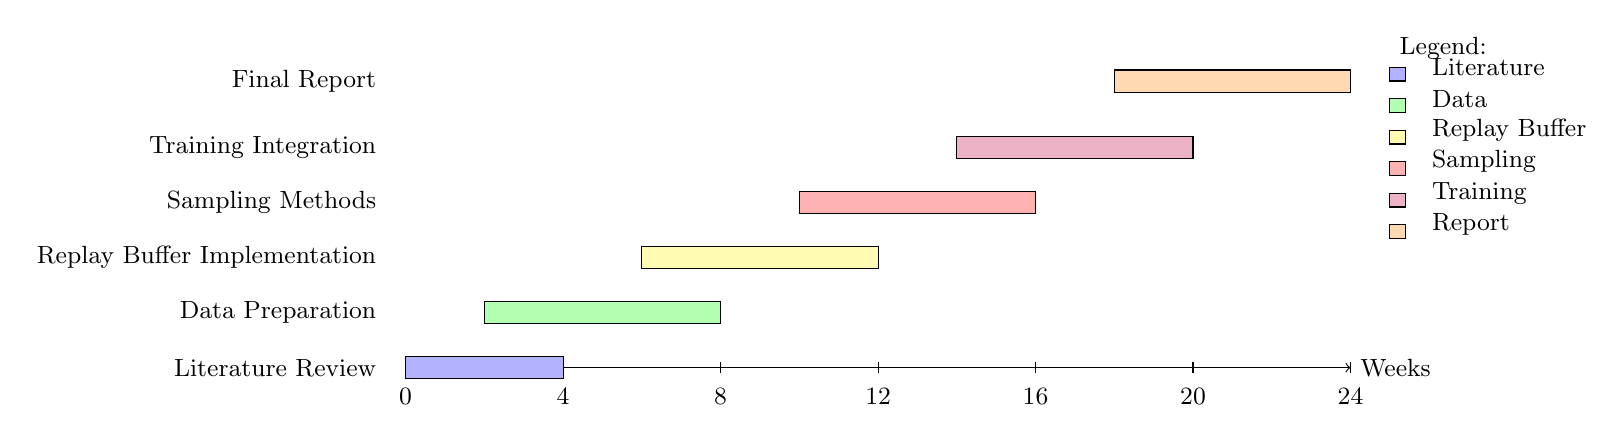
\begin{tikzpicture}[x=0.5cm, y=0.7cm, every node/.style={font=\small}]
    % Timeline axis
    \draw[->] (0,0) -- (24,0) node[right] {Weeks};
    % ticks and labels (fewer to avoid overlap)
    \foreach \x/\lbl in {0/0,4/4,8/8,12/12,16/16,20/20,24/24} {
        \draw (\x,-0.1) -- (\x,0.1);
        \node[below=2pt] at (\x,-0.1) {\lbl};
    }

    % Tasks (increased vertical spacing and left-aligned)
    \node[left] at (-0.5,5.2) {Final Report};
    \draw[fill=orange!30,draw=black] (18,5) rectangle (24,5.4);

    \node[left] at (-0.5,4) {Training Integration};
    \draw[fill=purple!30,draw=black] (14,3.8) rectangle (20,4.2);

    \node[left] at (-0.5,3) {Sampling Methods};
    \draw[fill=red!30,draw=black] (10,2.8) rectangle (16,3.2);

    \node[left] at (-0.5,2) {Replay Buffer Implementation};
    \draw[fill=yellow!30,draw=black] (6,1.8) rectangle (12,2.2);

    \node[left] at (-0.5,1) {Data Preparation};
    \draw[fill=green!30,draw=black] (2,0.8) rectangle (8,1.2);

    \node[left] at (-0.5,0) {Literature Review};
    \draw[fill=blue!30,draw=black] (0,-0.2) rectangle (4,0.2);

    % Legend (moved to top-right inside the figure)
    \begin{scope}[shift={(25,5.2)}]
        \node[anchor=west,font=\small] at (0,0.6) {Legend:};
        \draw[fill=blue!30,draw=black] (0,0) rectangle (0.4,0.25) node[right=0.6em,black,anchor=west] {Literature};
        \begin{scope}[yshift=-0.4cm]
            \draw[fill=green!30,draw=black] (0,0) rectangle (0.4,0.25) node[right=0.6em,black,anchor=west] {Data};
        \end{scope}
        \begin{scope}[yshift=-0.8cm]
            \draw[fill=yellow!30,draw=black] (0,0) rectangle (0.4,0.25) node[right=0.6em,black,anchor=west] {Replay Buffer};
        \end{scope}
        \begin{scope}[yshift=-1.2cm]
            \draw[fill=red!30,draw=black] (0,0) rectangle (0.4,0.25) node[right=0.6em,black,anchor=west] {Sampling};
        \end{scope}
        \begin{scope}[yshift=-1.6cm]
            \draw[fill=purple!30,draw=black] (0,0) rectangle (0.4,0.25) node[right=0.6em,black,anchor=west] {Training};
        \end{scope}
        \begin{scope}[yshift=-2.0cm]
            \draw[fill=orange!30,draw=black] (0,0) rectangle (0.4,0.25) node[right=0.6em,black,anchor=west] {Report};
        \end{scope}
    \end{scope}
\end{tikzpicture}
\caption{Project Timeline Gantt Chart}
\label{fig:gantt}
\end{figure}

\subsection{References}
\bibliographystyle{plainnat}
\bibliography{litrev}

\newpage

\section{Literature Survey}

\subsection{Introduction to Sample Efficiency in Chess Evaluation Networks}

Chess evaluation networks have become essential components of modern chess engines, but their training efficiency remains a significant challenge. Traditional approaches sample training positions uniformly from game databases, but this fails to account for the fact that not all positions provide equal learning value. Some positions are more challenging and informative for the model, requiring prioritized attention during training.

This survey examines prioritized replay and non-IID sampling as key strategies for sample-efficient training of chess evaluation networks. Instead of uniform sampling under IID assumptions, these techniques use adaptive buffers that replay high-weighted positions more frequently, creating non-stationary training distributions that focus on challenging examples and break from traditional SGD assumptions. The field bridges reinforcement learning techniques with the unique challenges of combinatorial game positions.

Key terms include:
\begin{itemize}
    \item \textbf{Prioritized Replay}: Adaptive sampling that replays high-value examples more frequently
    \item \textbf{Non-IID Sampling}: Breaking from independent and identically distributed assumptions
    \item \textbf{Sample Weighting}: Functions that assign importance scores to training examples for replay prioritization
    \item \textbf{Naive Difficulty Scoring}: Simple heuristics for estimating example importance
    \item \textbf{Non-Stationary Distributions}: Training distributions that evolve and adapt during learning
\end{itemize}

\subsection{Key Themes in Sample-Efficient Chess Training}

\subsubsection{Prioritized Replay and Non-IID Sampling}

A key innovation in sample-efficient training is **prioritized replay**, where high-information positions are sampled more frequently than low-information ones, creating non-stationary training distributions. This breaks from the iid assumptions of traditional stochastic gradient descent and allows the training process to adaptively focus on currently challenging examples. Techniques include experience replay buffers with priority weighting and curriculum-based sampling that evolves the training distribution over time.

The core mechanism involves maintaining a replay buffer where positions are stored with associated weights. During training, positions are sampled proportionally to their weights, ensuring that high-value examples are revisited more often. This creates non-iid sampling patterns that adapt to the model's learning progress, prioritizing positions that currently provide the most learning signal.

Key challenges include designing appropriate weighting functions, managing buffer size and update frequency, and preventing overfitting to high-weighted examples. Advanced implementations incorporate dynamic weighting that adjusts based on training progress and ensemble disagreement measures.

\subsubsection{Sample Weighting Functions}

A critical aspect of prioritized replay is the design of weighting functions that estimate the importance of training examples. **Naive difficulty scoring** provides a starting point with simple heuristics like material imbalance or position complexity. More sophisticated approaches use information-theoretic measures such as gradient norms, ensemble disagreement, and predictive uncertainty. The key challenge is developing weighting functions that correlate well with actual learning value while being computationally tractable for frequent replay buffer updates.

\subsubsection{Information-Theoretic Training Objectives}

Research has explored various measures to quantify the informativeness of training positions within replay frameworks. Gradient-based scores measure how much a position affects network parameters, while ensemble disagreement identifies positions where different models make conflicting predictions. These scores help prioritize replay on positions that maximize learning progress and adapt the non-iid sampling distribution.

\subsubsection{Curriculum Learning and Synthetic Data}

Curriculum learning suggests training on progressively more complex positions, while synthetic data generation can create additional training examples. Within prioritized replay, these techniques help evolve the sampling distribution over time, starting with uniform sampling and gradually shifting to more focused non-iid patterns.

\subsection{Assessment and Relation to Project}

The literature reveals that sample efficiency in chess evaluation networks remains an open problem, with traditional uniform sampling far from optimal. While prioritized replay and non-IID sampling show significant promise for breaking from iid assumptions, their integration into coherent training strategies for chess is underexplored. My project will address this gap by developing prioritized replay buffers and non-IID sampling techniques that adaptively focus on challenging positions, with particular emphasis on dynamic weighting functions and non-stationary training distributions.

The key insight is that chess training can benefit greatly from non-iid sampling patterns that prioritize high-information positions through frequent replay. By implementing adaptive buffers that evolve the training distribution based on model progress, I will create training systems that break from traditional SGD assumptions and accelerate learning. This will build on recent advances in experience replay but apply them specifically to the combinatorial structure of chess through innovative weighting and sampling mechanisms.

Success will contribute to making strong chess evaluation more accessible through improved training efficiency, with potential applications to other domains requiring adaptive, non-stationary sampling from complex datasets.

\newpage

\section{Critical Comparison with ChatGPT}

\subsection{Prompts Used}

\textbf{Initial Prompt:} \\
"Write a literature survey on sample-efficient training methods for neural networks, focusing on different sample weighting functions and importance sampling techniques."

\textbf{Follow-up Prompt:} \\
"Expand on naive difficulty scoring and simple heuristics for estimating training example importance, and discuss how these compare to more sophisticated information-theoretic approaches in practice."

\subsection{AI-Generated Literature Survey}

[Insert ChatGPT output here]

\subsection{Observations on Quality and Accuracy}

The AI-generated survey provided a reasonable overview of generative modeling techniques but lacked depth in sample weighting functions and naive difficulty scoring approaches. While it correctly identified VAE and normalizing flows as relevant techniques, it oversimplified the practical challenges of implementing different weighting schemes and failed to discuss how simple heuristics compare to sophisticated information-theoretic measures. Citations were generally accurate but incomplete, missing some of the most relevant papers on importance sampling and adaptive weighting. The discussion of training efficiency was surface-level compared to the technical depth found in actual research on sample weighting and prioritized training.

\end{document}